\documentclass{article}
\usepackage{amsmath, amssymb}
\usepackage{mathhint}
\usepackage{pgfplots}
\pgfplotsset{compat=1.18}

\begin{document}

% Set the context for this problem - this information appears in the page header
% and helps the hint system understand what material you've covered
\mathhintcontext{
  book=Guckenheimer and Holmes,
  chapter=1,
  section=1.5-1.8,
  problem=1,
  lectures={lecture_5.tex, lecture_6.tex}
}

\begin{problem}
Consider the equations of motion for the simple pendulum with linear damping $\delta$ and constant applied torque $\beta$:
\[ \ddot{\theta}+\delta\dot{\theta}+\sin\theta=\beta \]
where $\delta,\beta\geq 0$ and $\theta$ is on the circle $S^1$ (which can be identified with the interval $[-\pi,\pi)$).
\begin{enumerate}
  \item[(a)] Find conditions on $(\beta,\delta)$ for which fixed points exist, linearize at the fixed points and draw conclusions on their stability types. Allow the parameters $(\beta,\delta)$ to vary, and locate values for which the linearizations are degenerate (non-hyperbolic).
  \item[(b)] For $\delta=0$, there is a conserved quantity (the system is Hamiltonian). Use this to deduce global phase portraits, and compare with information from (a).
  \item[(c)] For $\delta>0$, can this system have closed orbits that \textbf{do not} encircle the `phase cylinder'? [\textit{Hint:} Use Bendixson's criterion.]
  \item[(d)] For $\delta>0$ and $\beta>0$, can the system have closed orbits that \textbf{do} encircle the phase cylinder? [\textit{Hint:} Determine a trapping region and apply the Poincare-Bendixson theorem.]
\end{enumerate}

\end{problem}

\begin{notes}
\section{Part (a)}
Let's first rewrite our system into a two system ODE:
\begin{align*}
  \dot{\theta}&= \omega\\
  \dot{\omega}&= \beta -\delta \omega -\sin\theta
\end{align*}
To find fixed points, we can set these equations equal to 0:
\begin{align*}
  \dot{\theta}&= 0\\
  \dot{\omega}&=0= \beta -\delta \omega -\sin\theta=\beta -\delta \cdot 0 -\sin\theta
\end{align*}
Hence we have fixed points when
\[ \sin\theta = \beta \]
We can think about the number of fixed points and their positions as a horizontal line that starts at $\beta=-1$ and then sweeps to $\beta=+1$:
\begin{itemize}
  \item $\beta=-1$ --- There is one fixed point at $\arcsin(-1)=-\frac{\pi}{2}$.
  \item $-1<\beta\leq 0$ --- There are two fixed points with one in the range $[-\pi,-\pi / 2)$ and the other in the range $(-\pi / 2, 0]$.
  \item $0<\beta\leq 1$ --- There are two fixed points with one in the range $(0, \pi / 2)$ and the other in the range $(\pi / 2, \pi]$. Note that because of the boundary condition of $S^1$, the fixed point in $(\pi / 2, \pi)$ is a ``continuation'' of the fixed point previously from $[-\pi,-\pi / 2)$.
  \item $\beta=1$ --- There is one fixed point at $\arcsin(-1)=\frac{\pi}{2}$
\end{itemize}
\mathhint{Nudge}{2026-02-13 10:07}{You're on a good track finding the fixed points — now don't forget to linearize at each one by computing the Jacobian and analyzing its eigenvalues, which will tell you about stability and where degeneracies occur.}
Just to be explicit, we can write the fixed points $(\theta,\omega)$ as the following
\begin{itemize}
  \item $\beta=-1$ --- $(-\frac{\pi}{2},0)$
  \item $-1<\beta\leq 0$ --- $\left(\arcsin\beta,0\right),(-\pi-\arcsin\beta,0)$
  \item $0<\beta\leq 1$ --- $\left(\arcsin\beta,0\right),(\pi-\arcsin\beta,0)$
  \item $\beta=1$ --- $(\frac{\pi}{2},0)$
\end{itemize}
Note that we have to add the $\pm\pi$ values to the fixed points when $|\beta|<1$ because $\arcsin$ is only defined for $|x|\leq 1$ . Now let's linearize around each fixed point to determine their stability.

\subsection{$\beta=1$}

To linearize, we can compute the Jacobian 
\[ J_f(x,y) = \begin{bmatrix}
\frac{\partial f_1}{\partial \theta} & \frac{\partial f_1}{\partial \omega} \\
\frac{\partial f_2}{\partial \theta} & \frac{\partial f_2}{\partial \omega} 
\end{bmatrix} \]
with the quantities being 
\begin{gather*}
  \frac{\partial f_1}{\partial \theta}=0\\
  \frac{\partial f_1}{\partial \omega}=1\\
  \frac{\partial f_2}{\partial \theta}=-\cos\theta\\
  \frac{\partial f_2}{\partial \omega}=-\delta
\end{gather*}
For the case of $\beta=1$, we have 
\[
Df\left(\frac{\pi}{2},0\right)=\begin{bmatrix}
0 & 1 \\
-\cos\left(\frac{\pi}{2}\right) & -\delta
\end{bmatrix} = \begin{bmatrix}
0 & 1 \\
0 & -\delta
\end{bmatrix}
\]
For the eigenvalues and eigenvectors, we have 
\[
\left[ \left( \lambda_0 = 0, \  v_0=\left[ \left[\begin{matrix}1\\0\end{matrix}\right]\right]\right), \  \left( \lambda_1 = - \delta, \  v_1=\left[ \left[\begin{matrix}- \frac{1}{\delta}\\1\end{matrix}\right]\right]\right)\right]
\]
where a $\lambda_0 = 0$ tells us that this fixed-point is degenerate (non-hyperbolic).

\subsection{$-1<\beta\leq 0$}

We can use the same Jacobian as we computed in the $\beta=1$ case, but let's note some useful expressions:
\[
\cos\left(\arcsin \beta\right)=\sqrt{1-\sin\left(\arcsin\beta\right)^2}=\sqrt{1-\beta^2}
\]
For $\cos\left(\pm\pi-\arccos\beta\right)$, the expression is a bit more complicated, but we can make use of the identity $\cos(t-s)=\cos t \cos s + \sin t \cos s$:
\begin{align*}
  \cos\left(\pm\pi-\arccos\beta\right)&=\cos \left(\pm \pi\right) \cos\left(\arccos\beta\right) + \sin \left(\pm \pi\right) \cos \left(\arccos\beta\right)\\
  &=-1\cdot \cos\left(\arccos\beta\right)+0\cdot \cos \left(\arccos\beta\right)\\
  &=-\sqrt{1-\beta^2}
\end{align*}
For our fixed point $\left(\arcsin\beta,0\right)$, the Jacobian is 
\[
Df\left(\arcsin\beta,0\right)=\begin{bmatrix}
0 & 1 \\
-\cos\left(\arcsin\beta\right) & -\delta
\end{bmatrix} = \begin{bmatrix}
0 & 1 \\
-\sqrt{1-\beta^2} & -\delta
\end{bmatrix}
\]
Via SymPy, we get the following eigenvalues and eigenvectors
\[
\left(\lambda_0= - \frac{\delta}{2} - \frac{\sqrt{\delta^{2} - 4 \sqrt{1 - \beta^{2}}}}{2}, \ v_0=   \left[\begin{matrix}- \frac{\delta}{\sqrt{1 - \beta^{2}}} - \frac{\lambda_0}{\sqrt{1 - \beta^{2}}}\\1\end{matrix}\right]\right)
\]
and 
\[
 \left(\lambda_1= - \frac{\delta}{2} + \frac{\sqrt{\delta^{2} - 4 \sqrt{1 - \beta^{2}}}}{2}, \  v_1= \left[\begin{matrix}- \frac{\delta}{\sqrt{1 - \beta^{2}}} - \frac{\lambda_1}{\sqrt{1 - \beta^{2}}}\\1\end{matrix}\right]\right)
\]
Examining our eigenvalues, we only care about the sign of 
\[-\delta - \sqrt{\delta^{2} - 4 \sqrt{1 - \beta^{2}}}\qquad\text{and}\qquad -\delta + \sqrt{\delta^{2} - 4 \sqrt{1 - \beta^{2}}}\]
We have two cases: (1) the term $\sqrt{\delta^{2} - 4 \sqrt{1 - \beta^{2}}}$ is real and (2) the term $\sqrt{\delta^{2} - 4 \sqrt{1 - \beta^{2}}}$ is imaginary. In the case of (1), it necessarily follows that
\[\delta^2 > \delta^{2} - 4 \sqrt{1 - \beta^{2}},\]
hence we can state that $-\delta - \sqrt{\delta^{2} - 4 \sqrt{1 - \beta^{2}}}$ and $-\delta + \sqrt{\delta^{2} - 4 \sqrt{1 - \beta^{2}}}$ both have negative real parts, implying that $\left(\arcsin\beta,0\right)$ is a stable node. In the case of (2), it follows that $-\delta - \sqrt{\delta^{2} - 4 \sqrt{1 - \beta^{2}}}$ and $-\delta + \sqrt{\delta^{2} - 4 \sqrt{1 - \beta^{2}}}$ both have negative real parts, implying that $\left(\arcsin\beta,0\right)$ is a stable spiral. In fact, it is the value of $\delta$ that determines whether $\left(\arcsin\beta,0\right)$ is a stable spiral or stable node:
\begin{itemize}
  \item For $\delta^2 \geq 4 \sqrt{1 - \beta^{2}}$, we have a stable node 
  \item For $\delta^2 < 4 \sqrt{1 - \beta^{2}}$, we have a stable spiral
  \item For $\delta=0$, we have purely imaginary eigenvalues and linearization fails
\end{itemize}

\mathhint{Nudge}{2026-02-16 20:54}{You're making great progress with the linearization — now make sure to also analyze the *other* fixed point (the one at $-\pi - \arcsin\beta$ or $\pi - \arcsin\beta$) since it will have different stability properties due to the sign change in $\cos\theta$.}

For our fixed point $\left(-\pi - \arcsin\beta,0\right)$, the Jacobian is 
\[
Df\left(-\pi - \arcsin\beta,0\right)=\begin{bmatrix}
0 & 1 \\
-\cos\left(-\pi - \arcsin\beta\right) & -\delta
\end{bmatrix} = \begin{bmatrix}
0 & 1 \\
\sqrt{1-\beta^2} & -\delta
\end{bmatrix}
\]
Via SymPy, we get the following eigenvalues and eigenvectors
\[
\left(\lambda_0= - \frac{\delta}{2} - \frac{\sqrt{\delta^{2} + 4 \sqrt{1 - \beta^{2}}}}{2}, \ v_0=   \left[\begin{matrix}- \frac{\delta}{\sqrt{1 - \beta^{2}}} - \frac{\lambda_0}{\sqrt{1 - \beta^{2}}}\\1\end{matrix}\right]\right)
\]
and 
\[
 \left(\lambda_1= - \frac{\delta}{2} + \frac{\sqrt{\delta^{2} + 4 \sqrt{1 - \beta^{2}}}}{2}, \  v_1= \left[\begin{matrix}- \frac{\delta}{\sqrt{1 - \beta^{2}}} - \frac{\lambda_1}{\sqrt{1 - \beta^{2}}}\\1\end{matrix}\right]\right)
\]
Examining our eigenvalues, we only care about the sign of 
\[-\delta - \sqrt{\delta^{2} + 4 \sqrt{1 - \beta^{2}}}\qquad\text{and}\qquad -\delta + \sqrt{\delta^{2} + 4 \sqrt{1 - \beta^{2}}}\]
It clearly follows that $-\delta - \sqrt{\delta^{2} + 4 \sqrt{1 - \beta^{2}}}$ is a negative real number, and that 
\[\delta^2 < \delta^{2} + 4 \sqrt{1 - \beta^{2}},\]
hence $-\delta + \sqrt{\delta^{2} + 4 \sqrt{1 - \beta^{2}}}$ is a real positive number. Therefore, it follows that $\left(-\pi - \arcsin\beta,0\right)$ is a saddle node.

\subsection{$0<\beta\leq 1$}

Notice that our calculations for the fixed point $\left(\arcsin\beta,0\right)$ is the same as in $-1<\beta\leq 0$, and our calculation for the fixed point $\left(\pi - \arcsin\beta,0\right)$ is the same as $\left(-\pi - \arcsin\beta,0\right)$ since 
\[ 
\cos\left(\pm\pi-\arccos\beta\right)=  -\sqrt{1-\beta^2}
\]
Hence, $\left(\arcsin\beta,0\right)$ can either be a stable node or spiral depending on the value of $\delta$, and $\left(\pi - \arcsin\beta,0\right)$ is a saddle node.


\mathhint{Nudge}{2026-02-16 21:05}{You've done excellent work on part (a) — your analysis is thorough and correct. Now it's time to move on to part (b): think about what quantity is conserved when $\beta = 0$ and $\delta = 0$, and how its level curves give you the phase portrait.}

NOTE TO SELF: Need to mention when $\delta=0$.

\section{Part (b)}
To show that our system is Hamiltonian, we have to show there is a function $H(x,y)$ such that
\begin{align*}
  \dot{\theta}&=\frac{\partial H}{\partial \omega}\\
  \dot{\omega}&=-\frac{\partial H}{\partial \theta}.
\end{align*}
Starting with $\dot{\theta}$, we can write 
\begin{gather*}
  \frac{\partial H}{\partial \omega}=\omega\\
  \partial H=\omega\partial \omega\\
  \int \partial H = \int \omega\partial \omega\\
  H(\theta,\omega)=\frac{\omega^2}{2}+f(\theta)+C
\end{gather*}
Moving on to $\dot{\omega}$, we can write 
\begin{gather*}
  -\frac{\partial H}{\partial \theta}=\beta -\sin\theta\\
  \partial H = \left(\sin\theta- \beta\right)\partial \theta\\
  \int\partial H = \int\left(\sin\theta- \beta\right)\partial \theta\\
  H(\theta,\omega)=-\cos\theta -\frac{\beta^2}{2}+g(\omega)+C
\end{gather*}
Putting the two expressions together, we get 
\[
H(\theta,\omega) = -\cos\theta -\frac{\beta^2}{2}+\frac{\omega^2}{2}+C
\]
To get an expression for $C$, we can plug in for our fixed point $\left(\arcsin\beta,0\right)$, getting 
\begin{align*}
  H\left(\arcsin\beta,0\right) &= -\cos\left(\arcsin\beta\right)-\frac{\beta^2}{2}+\frac{0^2}{2}\\
  &= -\sqrt{1-\beta^2}-\frac{\beta^2}{2}
\end{align*}
Can this be reduced in any way?

\mathhint{Nudge}{2026-02-16 21:36}{You're on the right track with the Hamiltonian — but re-read the problem statement for part (b): it specifies $\delta = 0$ **and** $\beta = 0$, which simplifies your conserved quantity considerably. Then sketch the level curves of that simpler $H(\theta, \omega)$ to get the phase portrait.}

Huh, I guess since we found the Hamiltonian, we can just say that solutions follow level sets and then argue for the center at $\left(\arcsin\beta,0\right)$ and the homoclinic orbit at $\left(\pi-\arcsin\beta,0\right)$.

Wait, this isn't correct. My derivation of $f(\theta)$ has a error. It should have been 
\begin{gather*}
  -\frac{\partial H}{\partial \theta}=\beta -\sin\theta\\
  \partial H = \left(\sin\theta- \beta\right)\partial \theta\\
  \int\partial H = \int\left(\sin\theta- \beta\right)\partial \theta\\
  H(\theta,\omega)=-\cos\theta -\beta\theta+g(\omega)+C
\end{gather*}
meaning that the Hamiltonian is 
\[
H(\theta,\omega) = -\cos\theta -\beta\theta+\frac{\omega^2}{2}+C
\]

Via office hours, I learned that this problem is not asking about stability. We are tasked with finding the Hamiltonian, and then plotting level sets of the Hamiltonian for various energy values. We can find the homoclinic orbit by solving for the level set at that particular energy value.

\section{Part (c)}

Given that $\theta$ is on the circle $S^1$, the length of our cylinder is $\omega$. What the problem is asking is whether there are any closed orbits with $\theta$ contained within $S^1$. The hint to use Bendixson's criterion is suggesting that we use Bendixson's criterion to rule out periodic orbits, thus making it impossible that there are closed orbits, and hence, closed orbits that encircle the `phase cylinder'.

\mathhint{Nudge}{2026-02-16 22:04}{You're heading in the right direction with Bendixson's criterion — just compute $\nabla \cdot f$ for your vector field and see what it tells you when $\delta > 0$.}

Computing $\nabla\cdot(f,g)$, we have 
\begin{align*}
  \nabla\cdot(f,g)&=\partial_\theta \omega+\partial_\omega\left(\beta-\delta\omega-\sin\theta\right)\\
  &=0-\delta\\
  &=-\delta
\end{align*}
Via Bendixson's criterion, this system can only have periodic orbits if $\nabla\cdot(f,g)$ equals zero or changes sign. In our case, $\nabla\cdot(f,g)$ can only equal zero if $\delta=0$. Hence, the system can have closed orbits that do not encircle the `phase cylinder' only if $\delta=0$.


\mathhint{Nudge}{2026-02-17 07:46}{You've correctly handled part (c) — nice work with Bendixson's criterion. For part (d), think about what "encircling the phase cylinder" means in terms of $\theta$ and how the Poincaré-Bendixson theorem might apply if you can find a region that trajectories can't escape.}

Need to make some note about simply connected sets, and how you can't have a simply connected set wrap around the phase cylinder.

\section{Part (d)}

In line with the hint, the outline of the answer is to define a trapping region on $\omega$ and then use Poincaré-Bendixson theorem to argue there is a closed orbit. The trapping region on $\omega$ can be found by realizing the the $-\sin\theta$ term in $\dot{\omega}$ is bound by $+1$. Hence, we need to satisfy   
\[0>\dot{\omega}=\beta-\delta\omega+1\]
and so we can write 
\[ \omega>\frac{\beta+1}{\delta} \]
Hence if we have an initial $\omega(0)$ greater than $\frac{\beta+1}{\delta}$, regardless of $\theta$, $\dot{\omega}$ is negative. For the lower bound, we need to find $\dot{omega}>0$, hence we can write 
\[
\beta-\delta\omega+1=\dot{\omega}>0
\]
and we have 
\[
\frac{\beta+1}{\delta} > \omega
\]
Wait this reasoning feels horribly circular. What did I do wrong?

\mathhint{Nudge}{2026-02-19 14:26}{You're close — check the lower bound more carefully. For $\dot{\omega} > 0$, you need the *worst case* of $-\sin\theta$, which gives you a *different* bound than the upper case.}

In line with the hint, the outline of the answer is to define a trapping region on $\omega$ and then use Poincaré-Bendixson theorem to argue there is a closed orbit. The trapping region on $\omega$ can be found by realizing the the $-\sin\theta$ term in $\dot{\omega}$ is bound by $+1$ and $-1$. To find an upper bound such that $0>\dot{\omega}$, we need to satisfy   
\[0>\dot{\omega}=\beta-\delta\omega+1\]
and so we can write 
\[ \omega>\frac{\beta+1}{\delta} \]
Hence if we have an initial $\omega(0)$ greater than $\frac{\beta+1}{\delta}$, regardless of $\theta$, $\dot{\omega}$ is negative. For the lower bound, we need to find $\dot{omega}>0$, hence we can write 
\[
\beta-\delta\omega-1=\dot{\omega}>0
\]
and we have 
\[
\frac{\beta-1}{\delta} > \omega
\]
Therefore, we have a trapping region 
\[ U=[\frac{\beta-1}{\delta} - \epsilon, \frac{\beta+1}{\delta}+\epsilon ] \]
for some $\epsilon>0$.

\mathhint{Nudge}{2026-02-19 14:52}{You're on the right track with the trapping region — now think carefully about what lives inside that region and how the Poincaré-Bendixson theorem applies on the cylinder to conclude the existence of a closed orbit encircling it.}

Note that this region $U$ wraps around the cylinder, hence it is possible to get orbits that flow such that $\theta$ increases but can come back around to meet themselves. Also note that for $\beta>1$ in part (a), we showed that the system had no fixed points. Hence, via the Poincaré-Bendixson theorem, for $\beta>1$, we can conclude that a closed orbit exists within $U$.

\mathhint{Nudge}{2026-02-19 14:59}{You're almost there — but consider whether the conclusion is limited to $\beta > 1$. Think about what happens when $0 < \beta \leq 1$: there are fixed points, but do any of them actually lie *inside* your trapping region $U$?}

When $0<\beta<1$ then our lower bound is negative; hence, the fixed points are included in the trapping region $U$. What does that tell us?

\mathhint{Nudge}{2026-02-19 16:40}{Think about *where* those fixed points sit — what are their $\omega$-coordinates, and does that actually place them inside the strip $U$?}

The fixed points sit at $\omega=0$, as we established in part (a). Therefore, any lower bound on $\omega$ that is negative will include the fixed points.

\mathhint{Nudge}{2026-02-19 16:43}{The fixed points are at $\omega = 0$, and your lower bound is $\frac{\beta - 1}{\delta}$, which is negative when $0 < \beta < 1$ — so yes, they're inside $U$. But can you modify the trapping region to *exclude* them, perhaps by raising the lower bound on $\omega$ above zero?}
\mathhint{Direction}{2026-02-19 16:55}{Consider whether a strip of the form $U = \{\omega_{\min} \leq \omega \leq \omega_{\max}\}$ with $\omega_{\min} > 0$ can still be made into a trapping region — check what $\dot{\omega}$ looks like when $\omega$ is small but positive, and whether the flow still points inward on that lower boundary.}

Wait, but doesn't the problem just ask ``can the system...'' because in this case, we've clearly shown that the system ``can'' have a closed orbit that does encircle the phase cylinder. We provided and existence proof of at least one case where there is such an orbit.

\mathhint{Nudge}{2026-02-19 17:09}{You're right — for $\beta > 1$ your argument is already complete and sufficient to answer "yes, it can." If you want to strengthen your answer, you could also address the $0 < \beta \leq 1$ case, but your existing proof is a valid answer to the question as posed.}
\end{notes}

\begin{solution}

\section{Part (a)}
Let's first rewrite our system into a two system ODE:
\begin{align*}
  \dot{\theta}&= \omega\\
  \dot{\omega}&= \beta -\delta \omega -\sin\theta
\end{align*}
To find fixed points, we can set these equations equal to 0:
\begin{align*}
  \dot{\theta}&= 0\\
  \dot{\omega}&=0= \beta -\delta \omega -\sin\theta=\beta -\delta \cdot 0 -\sin\theta
\end{align*}
Hence we have fixed points when
\[ \sin\theta = \beta \]
We can think about the number of fixed points and their positions as a horizontal line that starts at $\beta=0$ and then sweeps to $\beta=+1$:
\begin{itemize}
  \item $\beta= 0$ --- There are two fixed points with one at $\theta=-\pi$ and the other in at $\theta=0$.
  \item $0<\beta\leq 1$ --- There are two fixed points with one in the range $\theta\in(0, \pi / 2)$ and the other in the range $\theta\in(\pi / 2, \pi)$. Note that because of the boundary condition of $S^1$, the fixed point in $\theta\in(\pi / 2, \pi)$ is a ``continuation'' of the fixed point previously from $\theta=-\pi,$.
  \item $\beta=1$ --- There is one fixed point at $\theta=\arcsin(-1)=\frac{\pi}{2}$
\end{itemize}
To be explicit, we can write the fixed points $(\theta,\omega)$ as the following
\begin{itemize}
  \item $\beta=0$ gives us $(-\pi,0),(0,0)$
  \item $0<\beta\leq 1$ gives us $\left(\arcsin\beta,0\right),(\pi-\arcsin\beta,0)$
  \item $\beta=1$ gives us $(\frac{\pi}{2},0)$
\end{itemize}
Note that we have to add the $\pm\pi$ values to the fixed points when $|\beta|<1$ because $\arcsin$ is only defined for $|x|\leq 1$ . Now let's linearize around each fixed point to determine their stability. 

To linearize, we can compute the Jacobian 
\[ J_f(x,y) = \begin{bmatrix}
\frac{\partial f_1}{\partial \theta} & \frac{\partial f_1}{\partial \omega} \\
\frac{\partial f_2}{\partial \theta} & \frac{\partial f_2}{\partial \omega} 
\end{bmatrix} \]
with the quantities being 
\begin{gather*}
  \frac{\partial f_1}{\partial \theta}=0\\
  \frac{\partial f_1}{\partial \omega}=1\\
  \frac{\partial f_2}{\partial \theta}=-\cos\theta\\
  \frac{\partial f_2}{\partial \omega}=-\delta
\end{gather*}

Before we focus on fixed points, let's note some useful expressions:
\[
\cos\left(\arcsin \beta\right)=\sqrt{1-\sin\left(\arcsin\beta\right)^2}=\sqrt{1-\beta^2}
\]
For $\cos\left(\pm\pi-\arccos\beta\right)$, the expression is a bit more complicated, but we can make use of the identity $\cos(t-s)=\cos t \cos s + \sin t \cos s$:
\begin{align*}
  \cos\left(\pm\pi-\arccos\beta\right)&=\cos \left(\pm \pi\right) \cos\left(\arccos\beta\right) + \sin \left(\pm \pi\right) \cos \left(\arccos\beta\right)\\
  &=-1\cdot \cos\left(\arccos\beta\right)+0\cdot \cos \left(\arccos\beta\right)\\
  &=-\sqrt{1-\beta^2}
\end{align*}

Now dealing with the case of $\beta=0$, we can start with the fixed point $(0,0)$. The Jacobian is 
\[ Df(0,0) = \begin{bmatrix}
0 & 1 \\
-1 & -\delta
\end{bmatrix} \]
Via SymPy, we get the following eigenvalues
\[
\lambda_0 = - \frac{\delta}{2} - \frac{\sqrt{\delta^2 - 4}}{2}, \qquad \lambda_1 = - \frac{\delta}{2} + \frac{\sqrt{\delta^2 - 4}}{2}
\]
where we have three cases: (1) $\delta=0$, (2) $0<\delta<2$, (3) $\delta\geq2$.
\begin{enumerate}
  \item For $\delta=0$, both eigenvalues become $\lambda_0=-i,\lambda_1=+i$ and linearization tells us nothing. The fixed point is non-hyperbolic.
  \item For $0<\delta<2$, both eigenvalues are complex with negative real parts. Hence, $(0,0)$ is stable. In particular, it is a stable spiral.
  \item For $\delta\geq2$, both eigenvalues are real and negative. Note that $\lambda>\sqrt{\lambda^2-4}$ so $\lambda_1$ is indeed negative. Therefore, $(0,0)$ is stable. In particular, it is a stable node.
\end{enumerate}

Now continuing with $\beta=0$, we can move to the fixed point $(-\pi,0)$. The Jacobian is 
\[ Df(0,0) = \begin{bmatrix}
0 & 1 \\
1 & -\delta
\end{bmatrix} \]
Via SymPy, we get the following eigenvalues
\[
\lambda_0 = - \frac{\delta}{2} - \frac{\sqrt{\delta^{2} + 4}}{2}, \qquad \lambda_1 = - \frac{\delta}{2} + \frac{\sqrt{\delta^{2} + 4}}{2}
\]
where for all values of $\delta$, it follows that $\lambda_0$ is negative and $\lambda_1$ is positive (note that $\delta<\sqrt{\delta^2+4}$). Hence, $(-\pi,0)$ is a saddle.

Now dealing with the case of $0<\beta\leq 1$, we can start with the fixed point $\left(\arcsin\beta,0\right)$. The Jacobian is 
\[
Df\left(\arcsin\beta,0\right)=\begin{bmatrix}
0 & 1 \\
-\cos\left(\arcsin\beta\right) & -\delta
\end{bmatrix} = \begin{bmatrix}
0 & 1 \\
-\sqrt{1-\beta^2} & -\delta
\end{bmatrix}
\]
Via SymPy, we get the following eigenvalues and eigenvectors
\[
\left(\lambda_0= - \frac{\delta}{2} - \frac{\sqrt{\delta^{2} - 4 \sqrt{1 - \beta^{2}}}}{2}, \ v_0=   \left[\begin{matrix}- \frac{\delta}{\sqrt{1 - \beta^{2}}} - \frac{\lambda_0}{\sqrt{1 - \beta^{2}}}\\1\end{matrix}\right]\right)
\]
and 
\[
 \left(\lambda_1= - \frac{\delta}{2} + \frac{\sqrt{\delta^{2} - 4 \sqrt{1 - \beta^{2}}}}{2}, \  v_1= \left[\begin{matrix}- \frac{\delta}{\sqrt{1 - \beta^{2}}} - \frac{\lambda_1}{\sqrt{1 - \beta^{2}}}\\1\end{matrix}\right]\right)
\]
Examining our eigenvalues, we only care about the sign of 
\[-\delta - \sqrt{\delta^{2} - 4 \sqrt{1 - \beta^{2}}}\qquad\text{and}\qquad -\delta + \sqrt{\delta^{2} - 4 \sqrt{1 - \beta^{2}}}\]
We have two cases: (1) $\delta=0$ and linearization fails due to purely imaginary eigenvalues, (2) the term $\sqrt{\delta^{2} - 4 \sqrt{1 - \beta^{2}}}$ is real and (3) the term $\sqrt{\delta^{2} - 4 \sqrt{1 - \beta^{2}}}$ is imaginary. In the case of (2), it necessarily follows that
\[\delta^2 > \delta^{2} - 4 \sqrt{1 - \beta^{2}},\]
hence we can state that $-\delta - \sqrt{\delta^{2} - 4 \sqrt{1 - \beta^{2}}}$ and $-\delta + \sqrt{\delta^{2} - 4 \sqrt{1 - \beta^{2}}}$ both have negative real parts, implying that $\left(\arcsin\beta,0\right)$ is a stable node. In the case of (3), it follows that $-\delta - \sqrt{\delta^{2} - 4 \sqrt{1 - \beta^{2}}}$ and $-\delta + \sqrt{\delta^{2} - 4 \sqrt{1 - \beta^{2}}}$ both have negative real parts, implying that $\left(\arcsin\beta,0\right)$ is a stable spiral. In fact, it is the value of $\delta$ that determines whether $\left(\arcsin\beta,0\right)$ is a stable spiral or stable node:
\begin{itemize}
  \item For $\delta^2 \geq 4 \sqrt{1 - \beta^{2}}$, we have a stable node 
  \item For $\delta^2 < 4 \sqrt{1 - \beta^{2}}$, we have a stable spiral
  \item For $\delta=0$, we have purely imaginary eigenvalues and linearization fails. The fixed point is non-hyperbolic.
\end{itemize}

For our fixed point $\left(\pi - \arcsin\beta,0\right)$, the Jacobian is 
\[
Df\left(\pi - \arcsin\beta,0\right)=\begin{bmatrix}
0 & 1 \\
-\cos\left(\pi - \arcsin\beta\right) & -\delta
\end{bmatrix} = \begin{bmatrix}
0 & 1 \\
\sqrt{1-\beta^2} & -\delta
\end{bmatrix}
\]
Via SymPy, we get the following eigenvalues and eigenvectors
\[
\left(\lambda_0= - \frac{\delta}{2} - \frac{\sqrt{\delta^{2} + 4 \sqrt{1 - \beta^{2}}}}{2}, \ v_0=   \left[\begin{matrix}- \frac{\delta}{\sqrt{1 - \beta^{2}}} - \frac{\lambda_0}{\sqrt{1 - \beta^{2}}}\\1\end{matrix}\right]\right)
\]
and 
\[
 \left(\lambda_1= - \frac{\delta}{2} + \frac{\sqrt{\delta^{2} + 4 \sqrt{1 - \beta^{2}}}}{2}, \  v_1= \left[\begin{matrix}- \frac{\delta}{\sqrt{1 - \beta^{2}}} - \frac{\lambda_1}{\sqrt{1 - \beta^{2}}}\\1\end{matrix}\right]\right)
\]
Examining our eigenvalues, we only care about the sign of 
\[-\delta - \sqrt{\delta^{2} + 4 \sqrt{1 - \beta^{2}}}\qquad\text{and}\qquad -\delta + \sqrt{\delta^{2} + 4 \sqrt{1 - \beta^{2}}}\]
It clearly follows that $-\delta - \sqrt{\delta^{2} + 4 \sqrt{1 - \beta^{2}}}$ is a negative real number, and that 
\[\delta^2 < \delta^{2} + 4 \sqrt{1 - \beta^{2}},\]
hence $-\delta + \sqrt{\delta^{2} + 4 \sqrt{1 - \beta^{2}}}$ is a real positive number. Therefore, it follows that $\left(\pi - \arcsin\beta,0\right)$ is a saddle for all values of $\delta$.

For the case of $\beta=1$, we have 
\[
Df\left(\frac{\pi}{2},0\right)=\begin{bmatrix}
0 & 1 \\
-\cos\left(\frac{\pi}{2}\right) & -\delta
\end{bmatrix} = \begin{bmatrix}
0 & 1 \\
0 & -\delta
\end{bmatrix}
\]
For the eigenvalues and eigenvectors, we have 
\[
\left[ \left( \lambda_0 = 0, \  v_0=\left[ \left[\begin{matrix}1\\0\end{matrix}\right]\right]\right), \  \left( \lambda_1 = - \delta, \  v_1=\left[ \left[\begin{matrix}- \frac{1}{\delta}\\1\end{matrix}\right]\right]\right)\right]
\]
where a $\lambda_0 = 0$ tells us that this fixed-point is degenerate (non-hyperbolic).

\section{Part (b)}

To show that our system is Hamiltonian, we have to show there is a function $H(x,y)$ such that
\begin{align*}
  \dot{\theta}&=\frac{\partial H}{\partial \omega}\\
  \dot{\omega}&=-\frac{\partial H}{\partial \theta}.
\end{align*}
Starting with $\dot{\theta}$, we can write 
\begin{gather*}
  \frac{\partial H}{\partial \omega}=\omega\\
  \partial H=\omega\partial \omega\\
  \int \partial H = \int \omega\partial \omega\\
  H(\theta,\omega)=\frac{\omega^2}{2}+f(\theta)
\end{gather*}
Moving on to $\dot{\omega}$, we can write 
\begin{gather*}
  -\frac{\partial H}{\partial \theta}=\beta -\sin\theta\\
  \partial H = \left(\sin\theta- \beta\right)\partial \theta\\
  \int\partial H = \int\left(\sin\theta- \beta\right)\partial \theta\\
  H(\theta,\omega)=-\cos\theta -\beta\theta+g(\omega)
\end{gather*}
meaning that the Hamiltonian is 
\[
H(\theta,\omega) = -\cos\theta -\beta\theta+\frac{\omega^2}{2}
\]

To deduce properties about the global phase portrait with the Hamiltonian, we can simply solve the Hamiltonian for different points in the phase plane, and then solve for $\omega$ in terms of $\theta$. Let's use the points $(-\pi,0),(\pi/2,0)$ for $\beta=0$ and write 
\begin{gather*}
  H(-\pi,0)=-\cos(-\pi)+0^2/2=1\\
  H(\pi/2,0)=-\cos(\pi/2)+0^2/2=0
\end{gather*}
and then solving for $\omega$, we have 
\begin{gather*}
  -\cos\theta +\frac{\omega^2}{2}=1\\
  \omega=\pm\sqrt{2\left(1+\cos\theta\right)}
\end{gather*}
and
\begin{gather*}
  -\cos\theta +\frac{\omega^2}{2}=0\\
  \omega=\pm\sqrt{2\left(\cos\theta\right)}
\end{gather*}

See Figure 1 where we plot these functions\footnote{Generative AI was used to produce the plot.}. We can see that the graph of our saddle $(-\pi,0)$ comes back around to meet it, indicating a homoclinic orbit, which makes sense for a Hamiltonian system. For $(\pi/2,0)$, the level set traces out a circle, suggesting that the point $(0,0)$ is Lyapunov stable. While our linearization of $(0,0)$ failed in part (a), these plots reveal that we have a center.

\begin{figure}[ht]
\centering
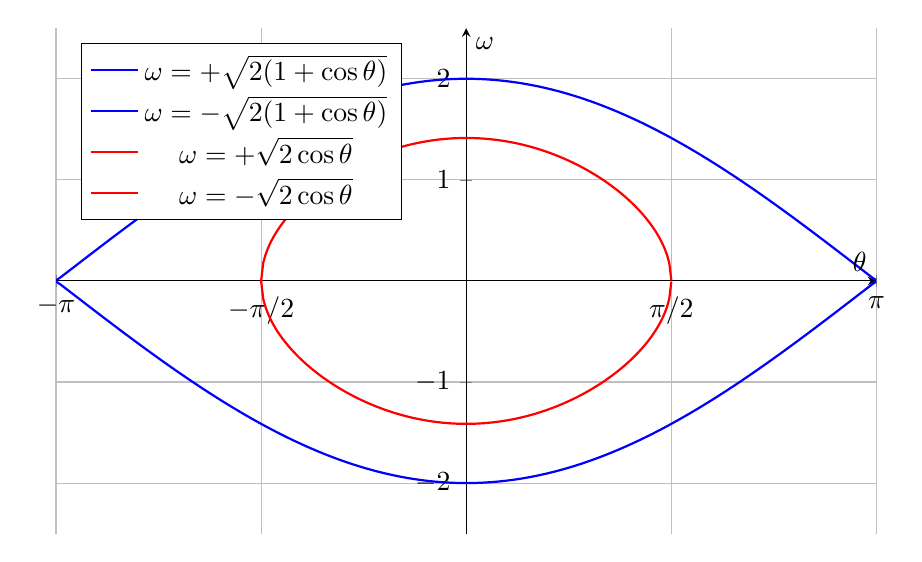
\begin{tikzpicture}
\begin{axis}[
    width=12cm,
    height=8cm,
    xlabel={$\theta$},
    ylabel={$\omega$},
    xmin=-pi, xmax=pi,
    ymin=-2.5, ymax=2.5,
    xtick={-pi, -pi/2, 0, pi/2, pi},
    xticklabels={$-\pi$, $-\pi/2$, $0$, $\pi/2$, $\pi$},
    grid=major,
    legend pos=north west,
    axis lines=center,
    samples=200,
    domain=-pi:pi,
]

% Upper branch: omega = sqrt(2(1+cos(theta)))
\addplot[blue, thick] {sqrt(2*(1+cos(deg(x))))};
\addlegendentry{$\omega=+\sqrt{2(1+\cos\theta)}$}

% Lower branch: omega = -sqrt(2(1+cos(theta)))
\addplot[blue, thick] {-sqrt(2*(1+cos(deg(x))))};
\addlegendentry{$\omega=-\sqrt{2(1+\cos\theta)}$}

% Upper branch: omega = sqrt(2*cos(theta)) for |theta| < pi/2
\addplot[red, thick, domain=-pi/2:pi/2] {sqrt(2*cos(deg(x)))};
\addlegendentry{$\omega=+\sqrt{2\cos\theta}$}

% Lower branch: omega = -sqrt(2*cos(theta)) for |theta| < pi/2
\addplot[red, thick, domain=-pi/2:pi/2] {-sqrt(2*cos(deg(x)))};
\addlegendentry{$\omega=-\sqrt{2\cos\theta}$}

\end{axis}
\end{tikzpicture}
\caption{Phase space trajectories}
\end{figure}

\section{Part (c)}

Given that $\theta$ is on the circle $S^1$, the length of our cylinder is $\omega$. What the problem is asking is whether there are any closed orbits with $\theta$ contained within $S^1$. The hint to use Bendixson's criterion is suggesting that we use Bendixson's criterion to rule out periodic orbits, thus making it impossible that there are closed orbits, and hence, closed orbits that encircle the `phase cylinder'. Note that Bendixson's criterion only applies for simply connected sets in our phase plane; however, this is requirement is met with the problem statement asking whether there are any closed orbits with $\theta$ contained within $S^1$. By focusing within $S^1$, we are constraining ourselves to only look at regions that can be described with simply connected sets.

Computing $\nabla\cdot(f,g)$, we have 
\begin{align*}
  \nabla\cdot(f,g)&=\partial_\theta \omega+\partial_\omega\left(\beta-\delta\omega-\sin\theta\right)\\
  &=0-\delta\\
  &=-\delta
\end{align*}
Via Bendixson's criterion, this system can only have periodic orbits if $\nabla\cdot(f,g)$ equals zero or changes sign. In our case, $\nabla\cdot(f,g)$ can only equal zero if $\delta=0$. Hence, the system can have closed orbits that do not encircle the `phase cylinder' only if $\delta=0$.

Moreover, we found such orbits in part (b) of this problem.

\section{Part (d)}

In line with the hint, our approach to the problem is to define a trapping region on $\omega$ and then use Poincaré-Bendixson theorem to argue there is a closed orbit. The trapping region on $\omega$ can be found by realizing the the $-\sin\theta$ term in $\dot{\omega}$ is bound by $+1$ and $-1$. To find an upper bound such that $0>\dot{\omega}$, we can set $\theta$ such that $-\sin\theta=+1$, and then write
\[0>\dot{\omega}=\beta-\delta\omega+1\]
where it implies that
\[ \omega>\frac{\beta+1}{\delta} \]
Hence if we have an initial $\omega(0)$ greater than $\frac{\beta+1}{\delta}$, regardless of $\theta$, $\dot{\omega}$ is negative. For the lower bound, we need to find $\dot{omega}>0$, hence we set $\theta$ such that $-\sin\theta=-1$ and write
\[
\beta-\delta\omega-1=\dot{\omega}>0
\]
where we have
\[
\frac{\beta-1}{\delta} > \omega
\]
Hence if we have an initial $\omega(0)$ less than $\frac{\beta-1}{\delta}$, regardless of $\theta$, $\dot{\omega}$ is positive. Therefore, we have a trapping region 
\[ U=\left\{(\theta,\omega): \omega\in\left[\frac{\beta-1}{\delta} - \epsilon, \frac{\beta+1}{\delta}+\epsilon \right] \right\}
\]
for some $\epsilon>0$. Also note that $U$ wraps around that phase cylinder in the $\theta$ direction, hence it is a compact set.

By setting $\beta>1$, part (a) tells us that there are no fixed points in the system; hence, there would be no fixed points in $U$. Therefore, applying Poincaré-Bendixson theorem, we can deduce that there must be a closed orbit in $U$.

\end{solution}

\end{document}
